\documentclass[english,notitlepage,reprint,nofootinbib]{revtex4-1}  % defines the basic parameters of the document
% For preview: skriv i terminal: latexmk -pdf -pvc filnavn
% If you want a single-column, remove "reprint"

% Allows special characters (including æøå)
\usepackage[utf8]{inputenc}
% \usepackage[english]{babel}

%% Note that you may need to download some of these packages manually, it depends on your setup.
%% I recommend downloading TeXMaker, because it includes a large library of the most common packages.

\usepackage{physics,amssymb}  % mathematical symbols (physics imports amsmath)
\include{amsmath}
\usepackage{graphicx}         % include graphics such as plots
\usepackage{xcolor}           % set colors
\usepackage{hyperref}         % automagic cross-referencing
\usepackage{listings}         % display code
\usepackage{subfigure}        % imports a lot of cool and useful figure commands
% \usepackage{float}
%\usepackage[section]{placeins}
\usepackage{algorithm}
\usepackage[noend]{algpseudocode}
\usepackage{subfigure}
\usepackage{tikz}
\usepackage{mathrsfs}

\usetikzlibrary{quantikz}
% defines the color of hyperref objects
% Blending two colors:  blue!80!black  =  80% blue and 20% black
\hypersetup{ % this is just my personal choice, feel free to change things
    colorlinks,
    linkcolor={red!50!black},
    citecolor={blue!50!black},
    urlcolor={blue!80!black}}


% ===========================================


\begin{document}

\title{A study of phase transition in the 2D Ising model\\through Markov Chain Monte Carlo simulation}  % self-explanatory
\author{Alessio Canclini, Filip von der Lippe} % self-explanatory
\date{\today}                             % self-explanatory
\noaffiliation                            % ignore this, but keep it.

%This is how we create an abstract section.
\begin{abstract}
    NB! Abstract here
\end{abstract}
\maketitle


% ===========================================
\section{Introduction}
This report will explore temperature-dependent behavior in ferromagnetism using the two-dimensional \textbf{Ising model}. The main purpose is determining a numerical estimation of the \textbf{critical temperature} at which the system transitions from a magnetized to a non-magnetized phase.

The Ising model is a widely studied model in statistical physics. Work on the Ising model has shown to be usfull for the analysis of several complex systems 

... more about Ising model and phase transitions
+ Mote Carlo methods and Markov chains. \cite{compendium}

% ===========================================
\section{Methods}\label{sec:methods}
The square 2D lattices for our Ising model will have a length of $L$ containing $N$ spins with the relation $N = L^2$. Each spin $s_i$ will have two possible states of 
\begin{equation*}
    s_i = -1 \text{ or } s_i = +1.
\end{equation*}
The total spin state or \textbf{spin configuration} of a lattice will be represented as $\textbf{s} = (s_1, s_2, ..., s_N)$. In its simplest form the total energy of the system is expressed as
\begin{equation*}
    E(\textbf{s}) = - J \sum^N_{\langle kl \rangle} s_k s_l - \mathscr{B} \sum^N_{k} s_k.
\end{equation*}
Here $\mathscr{B}$ is an external magnetic field. Since we will be looking at the Ising model without an external magnetic field the equation will be simplified to
\begin{equation}
    E(\textbf{s}) = - J \sum^N_{\langle kl \rangle} s_k s_l,
\end{equation}
where $\langle kl \rangle$ denotes the sum going over all \textit{neighboring pairs} of spins avoiding double-counting. $J$ is the \textbf{coupling constant} simply setting the energy associated with spin interactions. \textit{Periodic boundary conditions} will be implemented allowing all spins to have four neighbors.
\begin{equation}
    M(\textbf{s}) = \sum^N_i s_i
\end{equation}
is the magnetization of the entire system expressed as a sum over all spins. The energy per spin is
\begin{equation}
    \epsilon(\textbf{s}) = \frac{E(\textbf{s})}{N} \label{eq:mean_E}
\end{equation}
and the magnetization per spin is given by
\begin{equation}
    m(\textbf{s}) = \frac{M(\textbf{s})}{N}. \label{eq:mean_M}
\end{equation}
These will be used to compare and analyze results.
\begin{equation}
    \beta = \frac{1}{k_B T}
\end{equation}
describes the ``inverse temperature'' with the systems' temperature $T$ and the Boltzmann constant $k_B$.
\begin{equation}
    Z = \sum_{\text{all possible \textbf{s}}} e^{- \beta E(\textbf{s})}
\end{equation}
represents the partition function. This, the `inverse temperature'' and the total energy of the system appear in the \textit{Boltzmann distribution},
\begin{equation}
    p(\textbf{s};T) = \frac{1}{Z} e^{-\beta E(\textbf{s})}. \label{eq:prob_dist}
\end{equation}
This will be the probability distribution used for random sampling in our Monte Carlo approach. 


For comparison with early numerical implementations we will fist consider an analytical solution. The following table \ref*{tab:analytic} summarizes all sixteen possible \textbf{spin configurations} of a $2 \cross 2$ lattice with \textit{periodic boundary conditions}.

% Please add the following required packages to your document preamble:
% \usepackage[table,xcdraw]{xcolor}
% If you use beamer only pass "xcolor=table" option, i.e. \documentclass[xcolor=table]{beamer}
\begin{table}[H]
    \centering
    \begin{tabular}{|l|l|l|l|}
    \hline
    \begin{tabular}[c]{@{}l@{}}Nr. of spins \\ in state +1\end{tabular} & Degeneracy & \begin{tabular}[c]{@{}l@{}}Total \\ energy\end{tabular} & \begin{tabular}[c]{@{}l@{}}Total \\ magnetization\end{tabular} \\ \hline
    \hline
    0    & 1 & -8J & -4  \\    \hline
    1    & 4 & 0  & -2  \\    \hline
    2    & 4 & 0  & 0   \\    \hline
    2    & 2 & 8J  & 0   \\    \hline
    3    & 4 & 0  & 2   \\    \hline
    4    & 1 & -8J & 4   \\    \hline                                 
    \end{tabular} \label{tab:analytic}
    \caption{Analytic values for the sixteen \textbf{spin configurations} of the $2 \cross 2$ Ising model lattice.} 
\end{table} 
Based on the values in table \ref{tab:analytic} we derive the specific analytical expressions for the $2 \cross 2$ lattice case. The calculations of these analytic solutions can be found in appendix \ref{appendix:A} and are used to test early versions of the code.

We will study properties of the system at equilibrium for different lattice sizes as a function of temperature $T$. The analysis will focus on four main properties. The mean energy (eq. \ref{eq:mean_E}), mean magnetization (eq. \ref{eq:mean_M}), specific heat capacity
\begin{equation}
    C_V = \frac{1}{N} \frac{1}{k_B T^2} \left( \langle E^2 \rangle - \langle E \rangle^2 \right),
\end{equation}
and the susceptibility
\begin{equation}
    \chi = \frac{1}{N} \frac{1}{k_B T} \left( \langle M^2 \rangle - \langle |M| \rangle^2 \right).
\end{equation}
\subsection*{Periodic boundary conditions}
The Ising model simulations we will be implemented using periodic boundary conditions. This way, all spins will have four neighbors as seen in table \ref{tab:neighbors}, also at the boundaries of the lattice. NB! HOW ARE THESE IMPLEMENTED IN THE CODE.
\begin{table}[H]
    \centering
    \begin{tabular}{llll}
       & $\uparrow$ &    \\
    $\uparrow$ & $\uparrow$ & $\uparrow$ \\
       & $\uparrow$ & 
    \end{tabular}\label{tab:neighbors}
    \caption{An example of a spin and its neighbors. Here all five spins are in an up state (+1).} 
    \end{table}

\subsection*{Markov chain Monte Carlo method}
A Markov chain is a stok

\subsection*{The Metropolis algorithm}

\subsection*{Optimization and parallelization}

The Monte Carlo method will repeatedly require the Boltzmann factor $e^{-\beta \Delta E}$. The energy shift induced by flipping a single spin 
\begin{equation}
    \Delta E = E_{\text{after}} - E_{\text{before}}
\end{equation}
can only take five possible values in a 2D-lattice of arbitrary size($L > 2$) This is shown in appendix \ref{appendix:B}. These values are
\begin{equation}
    \Delta E = 8J, 4J, 0, -4J, -8J.
\end{equation}
To reduce computational cost we will avoid repeatedly calling the exponential function. This is done by pre-computing the five possible Boltzmann factors in an array. NB MORE HERE.

Furthermore, the code is written such that it can be run in series. This allows for easy parallelization using OpneMP to reduce runtimes.

% ===========================================
\section{Results}\label{sec:results}



% ===========================================
\section{Discussion}\label{sec:discussion}
%


% ===========================================
\section{Conclusion}\label{sec:conclusion}



\onecolumngrid

%\bibliographystyle{apalike}
\bibliography{ref}

\newpage
\appendix
\raggedbottom

\section{Analytical solutions for a 2$\cross$2 lattice}\label{appendix:A}
For the case of a 2$\cross$2 lattice with $L=2$ and $N=4$ we have sixteen possible spin configurations show in table \ref{tab:analytic}. These values will be used for the analytic solutions. The specific partition function becomes
\begin{align*}
    Z &=  \sum_{\text{all possible \textbf{s}}} e^{- \beta E(\textbf{s})} 
    = 2e^{- \beta (-8J)} + 2e^{- \beta 8J} + 12e^0 
    = 2 e^{\beta 8J} + 2 e^{- \beta 8J} + 12 
    = 4 (\cosh(8 \beta J) + 3).
\end{align*}
Additionally, we will calculate a few expectation values for which the general formula is given as
\begin{align*}
    \langle A \rangle = \sum_s A_s p(s).
\end{align*}
This is a sum over all spin states $s_i$. Here $p(s)$ is a chosen probability distribution, in our this case the Boltzmann distribution in eq. \ref{eq:prob_dist}. For the energy we have
\begin{align*}
    \langle E \rangle &=  \sum_s E(\textbf{s})  p(\textbf{s};T) 
    = \frac{1}{Z} \sum_s E(\textbf{s})  e^{-\beta E(\textbf{s})} 
    = \frac{1}{Z} \left( 2 \cdot (-8J)e^{\beta8J} + 2 \cdot 8J e^{-\beta 8J}\right) \\
    &= \frac{1}{Z} \left( -16 e^{\beta8J} + 16 e^{-\beta 8J}\right)
    = \frac{16J}{Z} \left( e^{-\beta 8J} - e^{\beta 8J} \right),
\\
\\
    \langle E^2 \rangle &=  \sum_s E(\textbf{s})^2  p(\textbf{s};T)
    = \frac{1}{Z} \sum_s E(\textbf{s})^2  e^{-\beta E(\textbf{s})} 
    = \frac{1}{Z} \left( 2 \cdot (-8J)^2e^{\beta8J} + 2 \cdot (8J)^2 e^{-\beta 8J}\right) \\
    &= \frac{128 J^2}{Z} \left( e^{-\beta 8J} + e^{\beta 8J} \right),
\\
\\
    \langle \epsilon \rangle &=  \sum_s \epsilon_s  p(\textbf{s};T)
    =  \sum_s \frac{E(\textbf{s})}{N}  p(\textbf{s};T)
    =  \frac{1}{N} \sum_s E(\textbf{s})  p(\textbf{s};T)
    =  \frac{\langle E \rangle }{4}
    = \frac{4J}{Z} \left( e^{-\beta 8J} - e^{\beta 8J} \right),
\\
\\
    \langle \epsilon^2 \rangle &=  \sum_s \epsilon_s^2  p(\textbf{s};T)
    =  \sum_s \left(\frac{E(\textbf{s})}{N}\right)^2  p(\textbf{s};T) 
    =  \frac{1}{N} \sum_s E(\textbf{s})^2  p(\textbf{s};T)
    =  \frac{\langle E^2 \rangle }{16}
    = \frac{8 J^2}{Z} \left( e^{-\beta 8J} + e^{\beta 8J} \right).
\end{align*}
Then for the magnetization we have
\begin{align*}
    \langle |M| \rangle &=  \sum_s |M(\textbf{s})|  p(\textbf{s};T) 
    = \frac{1}{Z} \sum_s |M(\textbf{s})| e^{-\beta E(\textbf{s})} 
    = \frac{1}{Z} \left( |-4|e^{\beta8J} + 4 |-2| e^0 + 4|2|e^0 + |4|e^{\beta 8J}\right) \\
    &= \frac{1}{Z} \left( 4e^{\beta8J} + 8 + 8 + 4e^{\beta 8J}\right)
    = \frac{8}{Z} \left( e^{\beta 8J} + 2 \right),
\\
\\
    \langle M^2 \rangle &= \sum_s M(\textbf{s})^2  p(\textbf{s};T) 
    = \frac{1}{Z} \sum_s M(\textbf{s})^2 e^{-\beta E(\textbf{s})} 
    = \frac{1}{Z} \left( (-4)^2 e^{\beta8J} + 4 (-2)^2 e^0 + 4(2)^2 e^0 + (4)^2 e^{\beta 8J}\right) \\
    &= \frac{1}{Z} \left( 16 e^{\beta8J} + 16 + 16 + 16 e^{\beta 8J}\right)
    = \frac{32}{Z} \left( e^{\beta 8J} + 1 \right),
\\
\\
    \langle |m| \rangle&= \sum_s |m(\textbf{s})|  p(\textbf{s};T) 
    = \frac{1}{Z} \sum_s \bigg| \frac{M(\textbf{s})}{N} \bigg| e^{-\beta E(\textbf{s})}
    = \frac{\langle|M| \rangle}{4}
    = \frac{2}{Z} \left( e^{\beta 8J} + 2 \right),
\\
\\
    \langle m^2 \rangle &= \sum_s m(\textbf{s})^2  p(\textbf{s};T)
    = \frac{1}{Z} \sum_s \left( \frac{M(\textbf{s})}{N} \right)^2 e^{-\beta E(\textbf{s})}
    = \frac{ \langle M^2 \rangle}{4^2}
    = \frac{ \langle M^2 \rangle}{16}
    = \frac{2}{Z} \left( e^{\beta 8J} + 1 \right).
\end{align*}

Finally, we find analytical expressions for the specific heat capacity
\begin{align*}
    C_V = \frac{1}{N} \frac{1}{k_B T^2} \left( \langle E^2 \rangle - \langle E \rangle^2 \right)
    = \frac{1}{4} \frac{1}{k_B T^2} \left( \frac{128 J^2}{Z} \left( e^{-\beta 8J} + e^{\beta 8J} \right) - \left( \frac{16J}{Z} \left( e^{-\beta 8J} - e^{\beta 8J} \right) \right)^2 \right)
    ,
\end{align*}
and the susceptibility
\begin{align*}
    \chi = \frac{1}{N} \frac{1}{k_B T} \left( \langle M^2 \rangle - \langle |M| \rangle^2 \right)
    = \frac{1}{4} \frac{1}{k_B T} \left( \frac{32}{Z} \left( e^{\beta 8J} + 1 \right) - \left( \frac{8}{Z} \left( e^{\beta 8J} + 2 \right) \right)^2 \right).
\end{align*}


\section{Possible $\Delta E$ values}\label{appendix:B}
Considering a 2D lattice of arbitrary size $(L>2)$ and remembering that we are working with periodic boundary conditions, we can show that there are only a few possible values of $\Delta E$. The calculation of $\Delta E$ between spin configurations will be limited to the flipping of a single spin. To find the possible energy differences we will look at a spin at a random position. This central spin will start in an up state(+1) and then be flipped (-1). We remind that $ E(\textbf{s}) = - J \sum^4_{\langle kl \rangle} s_k s_l$ and $ \Delta E = E_{\text{after}} - E_{\text{before}}$.
\begin{table}[H]
%\centering
\begin{tabular}{llll}
   & $\uparrow$ &    \\
$\uparrow$ & $\uparrow$ & $\uparrow$ \\
   & $\uparrow$ &  
\end{tabular}
has $E = -4J$, now flipping we have 
\begin{tabular}{llll}
    & $\uparrow$ &    \\
 $\uparrow$ & $\downarrow$ & $\uparrow$ \\
    & $\uparrow$ &  
 \end{tabular}
 and $E = 4J$, resulting in $\Delta E = 8J$.
\end{table}
This can be show for the four remaining possible starting configurations as well.
\begin{table}[H]
    %\centering
    \begin{tabular}{llll}
       & $\uparrow$ &    \\
    $\downarrow$ & $\uparrow$ & $\uparrow$ \\
       & $\uparrow$ &  
    \end{tabular}
    has $E = -2J$. Flipping we have 
    \begin{tabular}{llll}
        & $\uparrow$ &    \\
     $\downarrow$ & $\downarrow$ & $\uparrow$ \\
        & $\uparrow$ &  
     \end{tabular}
     and $E = 2J$, resulting in $\Delta E = 4J$.
\end{table}
    
\begin{table}[H]
    %\centering
    \begin{tabular}{llll}
       & $\uparrow$ &    \\
    $\downarrow$ & $\uparrow$ & $\uparrow$ \\
       & $\downarrow$ &  
    \end{tabular}
    has $E = 0$. Flipping we have 
    \begin{tabular}{llll}
        & $\uparrow$ &    \\
     $\downarrow$ & $\downarrow$ & $\uparrow$ \\
        & $\downarrow$ &  
     \end{tabular}
     and $E = 0$, resulting in $\Delta E = 0$.
\end{table}

\begin{table}[H]
    %\centering
    \begin{tabular}{llll}
       & $\uparrow$ &    \\
    $\downarrow$ & $\uparrow$ & $\downarrow$ \\
       & $\downarrow$ &  
    \end{tabular}
    has $E = 2J$. Flipping we have 
    \begin{tabular}{llll}
        & $\uparrow$ &    \\
     $\downarrow$ & $\downarrow$ & $\downarrow$ \\
        & $\downarrow$ &  
     \end{tabular}
     and $E = -2J$, resulting in $\Delta E = -4J$.
\end{table}

\begin{table}[H]
    %\centering
    \begin{tabular}{llll}
       & $\downarrow$ &    \\
    $\downarrow$ & $\uparrow$ & $\downarrow$ \\
       & $\downarrow$ &  
    \end{tabular}
    has $E = 4J$. Flipping we have 
    \begin{tabular}{llll}
        & $\downarrow$ &    \\
     $\downarrow$ & $\downarrow$ & $\downarrow$ \\
        & $\downarrow$ &  
     \end{tabular}
     and $E = -4J$, resulting in $\Delta E = -8J$.
\end{table}
The five possible values of the energy difference are thus, $\Delta E = 8J, 4J, 0, -4J, -8J$.

\section{Metropolis algorithm flow chart}\label{appendix:C}

\begin{figure}[H]
    \centering
    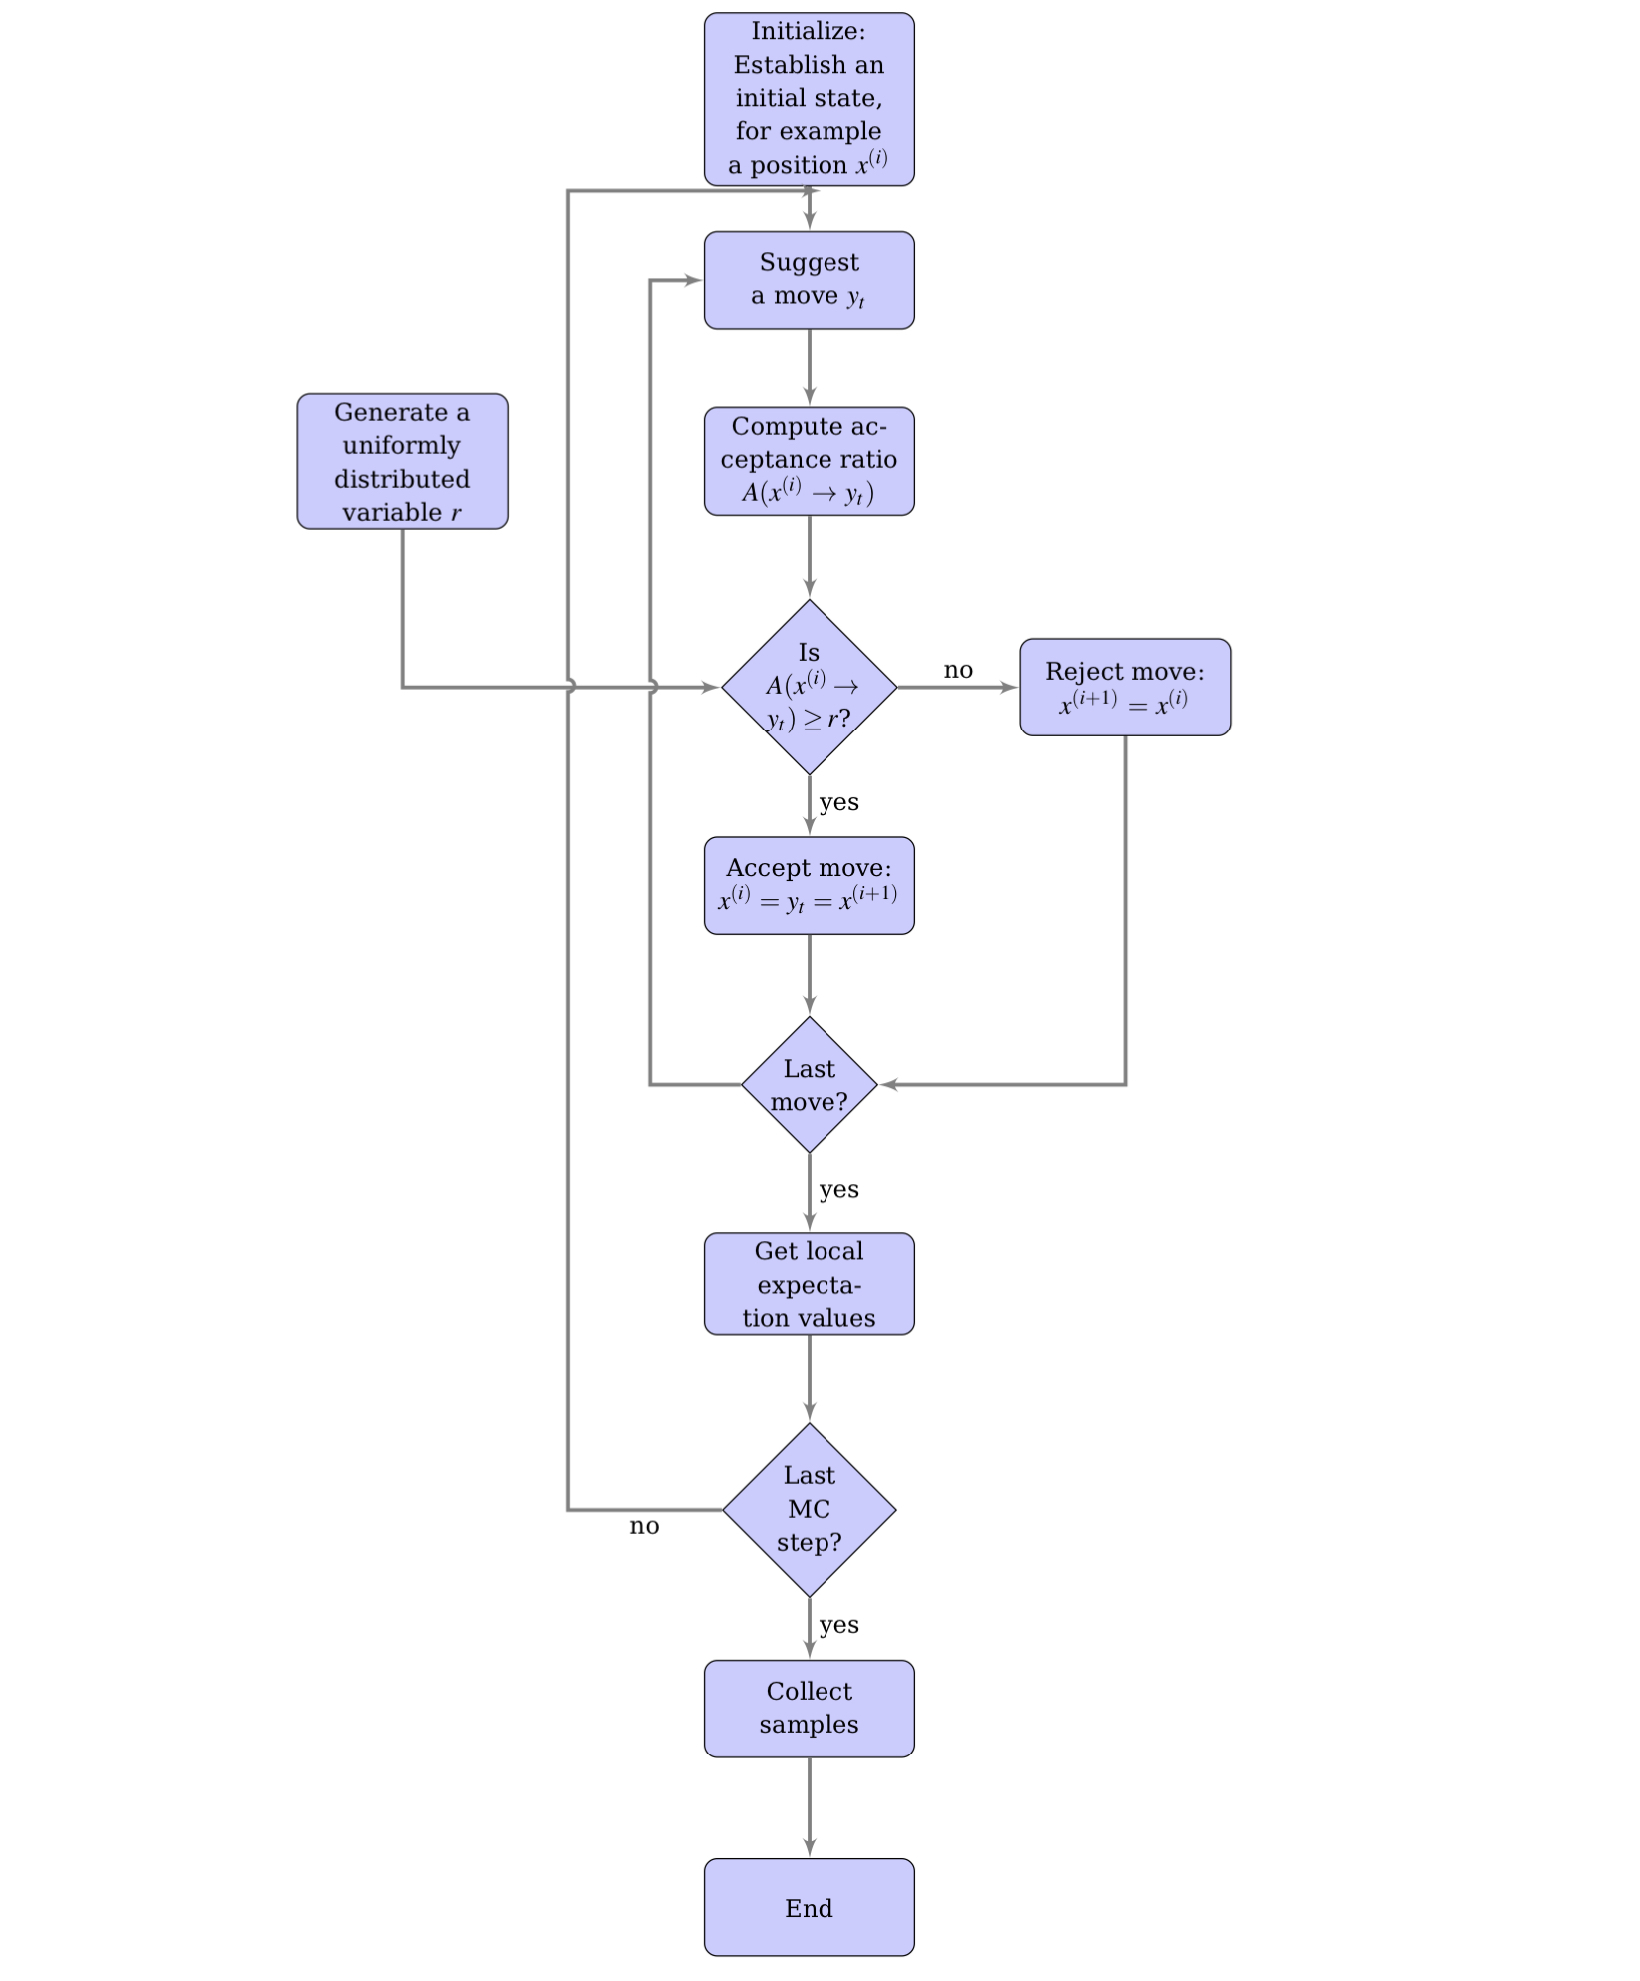
\includegraphics[width=1\textwidth]{../figures//metro_flow.jpg}
    \caption{Flowchart of the Metropolis algorithm taken from Computational Physics lecture notes \cite{compedium}.}
    \label{fig:metro_flow}
\end{figure}

\end{document}